\chapter{В поисках Юрковицы}

Сейчас горой Юрковицей считают склоны от Нижнеюрковской улицы в сторону к Мыльному переулку. Прежде, пока их не сожрали многочисленные заводы, пространство горы было больше, и занимало место, вписанное, по крайней мере, во всё пространство между Нижнеюрковской, Кирилловской и упомянутым переулком. После такого таяния горы, между склоном и Кирилловской улице, к нашему времени образовалась пустошь, огражденная от Кирилловской промзоной (бывший кирпичный завод, бывший пивзавод и т.д.), с карьерным озером на задворках. Полоса промзоны перестраивается в нечто иное, например в жилье.

Можно считать, что прежняя гора этом месте практически не сохранилась, она исчезла. Остались так, крайние высоты.

Эта же гора, в 18 веке, согласно земельным документам, именовалась Лысой и, насколько можно судить, Лисавицей. Подлинники я не видел, в передаче же печатным текстом разнобой - то гора Лысая, то Лисая, я не знаю как тогда произносили, не знаю и как именно было написано. Для удобства приму название Лысая. 

Известные мне документы 18 века не отражают гору под названием Юрковица, но есть соседствующий с Лысой Юрков ставок, из коего вытекал Юрков поток, вероятно затем преобразовавшийся в ручей Юрковицу.

Множество карт томятся в библиотеках и архивах, недоступные простым смертным. Я, простой смертный, могу рассуждать лишь на основании тех карт, кои пущены в обиход и которые можно рассмотреть. Например на плане конца 17 века Ушакова хоть и показаны интересующие нас склоны, имеющийся скан там попросту размыт (зачем тогда вообще было сканировать), а копии плана не отображают те места в нужной мере.

Доступный набор карт - а это по большому счету с середины 18 века - дает неоднозначную пищу для размышлений. И всё же важно выяснить, где именно находилась гора Юрковица, относилось ли вообще такое название к горе, если да, то не звалались ли она в летописные времена Хоревицей.

То, что современная Юрковица не называлась так в прошлом, доказывается ее прежним названием - Лысая. Однако там издавна было укрепленное поселение и погибло много людей. Позже я поведаю подробности.

Предполагаю, и по всей этой части книги поделюсь соображениями, что на этой Лысой горе стоял летописный град Киев, сооруженный Кием, Хоривом и Щеком в честь брата старшего.

Ученые никогда не рассматривали археологические находки на Лысой именно под таким углом, хотя находки эти подтверждают наличие тут древнего городища, а миниатюра из Радзивилловской летописи показывает «град Киев» здесь. Есть и другие доводы.

Но сперва кратко разберемся с обозначением горы Юрковицы и смежных с ней урочищ, важных для нас, на картах. Подробности же будут по мере продвижения по главам. Да, еще - иногда старинные карты нельзя точно наложить на современные, и чем глубже в прошлое, тем хуже это удается.

На плане 1752 года, показана "речка Юрковица" в пределах известного ныне в коллекторе одноименного ручья, а условно говоря южный склон вдоль верховий этой речки подписан "гора Щекавица". Если считать карту точной, то это обозначние относится к отрогу Щекавицы, где сейчас Старообрядческое кладбище. Минусы - карта весьма условна и скорее обозначает относительно расположение урочищ, я не смог ее порядком наложить на спутник.

Глубокое удолье, откуда вытекает "речка Юрковица", именуется на карта "Унизовая долина".

На весьма точном применительно к последующим векам плане Меленского 1803 года Юрковицей подписан современный угол между улицей Нижнеюрковской и Нижнеюрковским переулком.

Название Юрковицы пустилось в длинное путешествие, которое надо подробно осветить. На имеющихся у меня планах Киева, с 1803 по 1865 годы, Юрковицей подписана гора, которая теперь считается отрогом Щекавицы со старообрядческим кладбищем, то бишь холм, клином вписавшийся между улицей Нижнеюрковской и Нижнеюрковским переулком. Это же место будет в разных источниках проходить как Иорданские рогатки.

На плане 1833 года города Киева с проектом изменений, в тех местах неточном, о чем можно судить по половинам Иорданского кладище (они смещены), надпись "Юрковица" стоит поперек ставка, откуда истекает ручей Юрковица. Непонятно, относится ли надпись к ставку, или склону горы.

На плане 1837 года "урочище Юрковица" написано внизу на упомянутом перекрестке Нижнеюрковской улицы и переулка.

План 1845 года, "урочище Юрковица" - почти там же, но ближе к Кирилловской, малой частью на северо-восточном углу Щекавицы, и большей частью на юго-восточном углу Лысой горы между Кирилловской и Нижнеюрковской. Этот еще целый, неотгрызенный склон так показателен, что приведу иллюстрацию:

\begin{center}
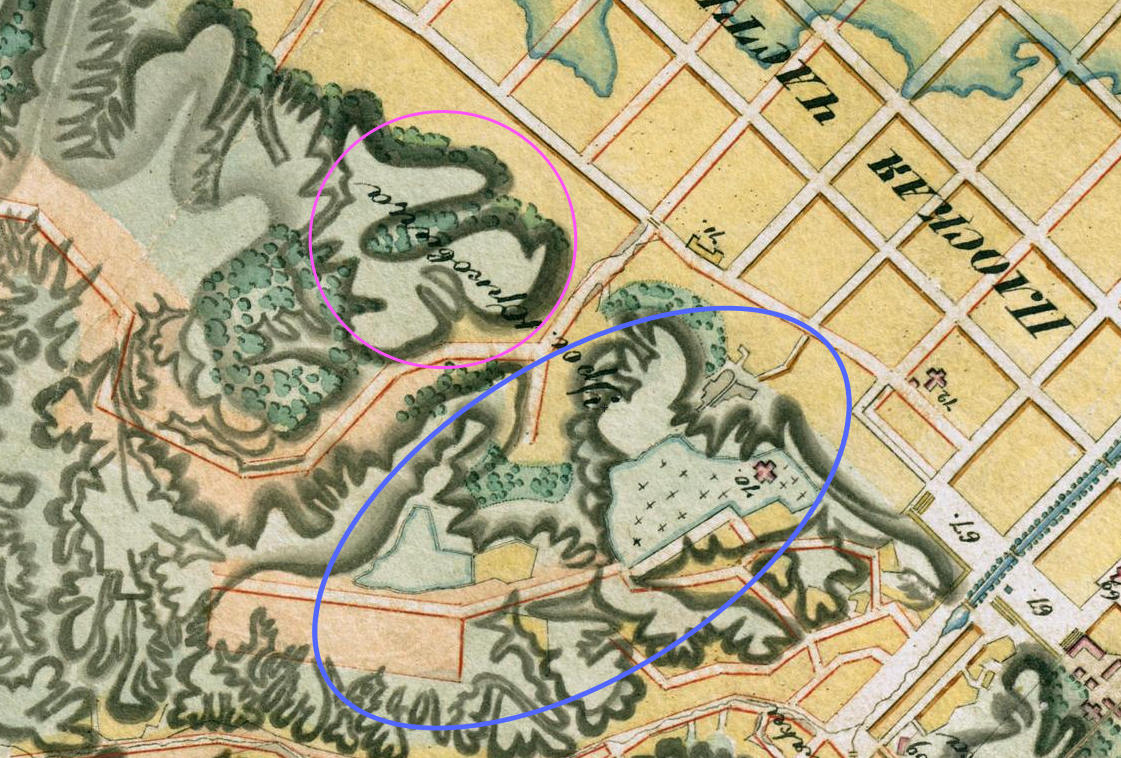
\includegraphics[width=\linewidth]{chast-kirvys/poisk-yourk/1845-marked.jpg}
\end{center} 

Синий овал - Щекавица, розовый - та часть Лысой горы, что подписана как "уроч. Юрковица", и весь ее склон вдоль Кирилловской, как видите, еще существует - а ныне там просто нет большей части горы, ее съели добычей глины.

На великолепной карте 1847 года "урочище Юрковица" раскинулось с отрога Щекавицы где Старобрядческие кладбище, на соседний склон Лысой горы, где в таком яру и был ставок, откуда вытекал ручей Юрковица. Если быть точным, то старообрядческое кладбище, ежели смотреть с юга на север, лежит в начале отрога, а северная часть отрога поныне ничем не занята и хранит следы давних валов и бассейна. Вот оттуда-то и распростерлась надпись "урочище Юрковица". Вот этот участок, ориентировано на север, всё легко находится по сохраняющемуся поныне перекрестку - "рогаткам".


\begin{center}
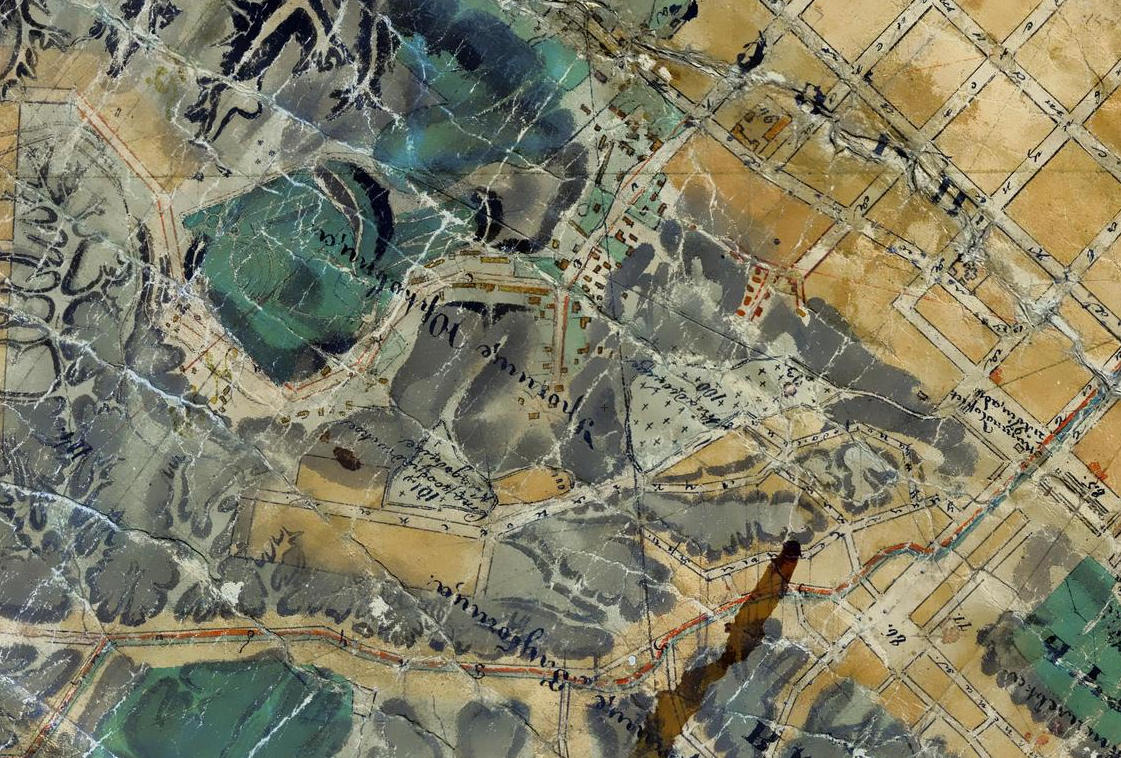
\includegraphics[width=\linewidth]{chast-kirvys/poisk-yourk/1847.jpg}
\end{cente




На карте 1880 года «Юрковица» прыгает на противоположную гору, а точнее на целый массив отрогов к северо-западу от Нижнеюрковской улицы. То же видим на карте 1882 года из энциклопедии «Britannica». А на замечательной в прочих отношениях карте 1886 года издания картографического заведения А. Ильина, этот же массив отрогов подписан «Щекавица». Сие повторено на французской карте 1896 года.

На многих планах названий гор вообще нет, есть впрочем «Щекавицкое кладбище». Затем на плане 1912 года мы снова видим надпись «Щекавица» там, где теперь на картах пишут «Юрковица», к северо-западу от Нижнеюрковской.

Наконец, на последней советской карте Киева, 1991 года, горы указаны хитро. Щекавица там, где Щекавица традиционно имеет место быть, то бишь гора, по которой идет улица Олеговская и стоит вышка. А вот Юрковица подписана к западу от «Щекавицы», и можно понимать и на месте исконной Юрковицы, и на месте котельной «Лукьяновская», еще западнее первоначальной Юрковицы. 

Такое впечатление, что картографами несколько веков упорно велась борьба по переносу Юрковицы на север, а потом с севера на прежнее, или почти прежнее положение. Примерно с начала 20 века, в народе Юрковицей слывет гора, примыкающая к северной, четной стороне улицы Нижнеюрковской. Эта гора в земельных документах 17-18 веков именовалась «Лысой», а еще раньше там был град Кия.

Я составил две карты, чтобы наглядно показать перенос названия от прежнего к современному. Контуры прорисованы мною по немецкой аэрофотосъемке времен Великой Отечественной войны. С тех пор мало что изменилось (кроме сильно сожранного кирпичным заводом юго-восточного склона Лысой горы), а мне было удобно, ибо на снимках четко виден рельеф. 

От улицы Кирилловской на запад в овраге отходит улица Нижнеюрковская. Раньше она именовалась Большой Юрковской или просто Юрковской. С этой Юрковской вообще связана большая путаница, которой мы коснемся по мере надобности. Покамест надо знать, что ныне Юрковская и Нижнеюрковская делятся по соприкосновению с Кирилловской.

От Нижнеюрковской вниз, к югу, отделяется Нижнеюрковский переулок, я его не подписал. Похоже на рогатку. Сия местность раньше так и называлась – Ерданские Рогатки. В середине 19 века, южная ветвь их именовалась Ближней или Нижней Юрковицей, а западная – Дальней, или Верхней Юрковицей.

Сейчас все отроги горы, что лежит к югу от Нижнеюрковской улицы, считаются Щекавицей. Однако на картах первой половины 19 века, северо-западный отрог (со старообрядческим кладбищем) подписан Юрковицей. Гора напротив него, к северу, в 17-18 веках называлась Лысой. 

На моей карте овал с подписью «град Кия» не означает, что град занимал именно такое положение и имел такой размер. Скорее, град Кия покрывал всю гору.

\begin{center}
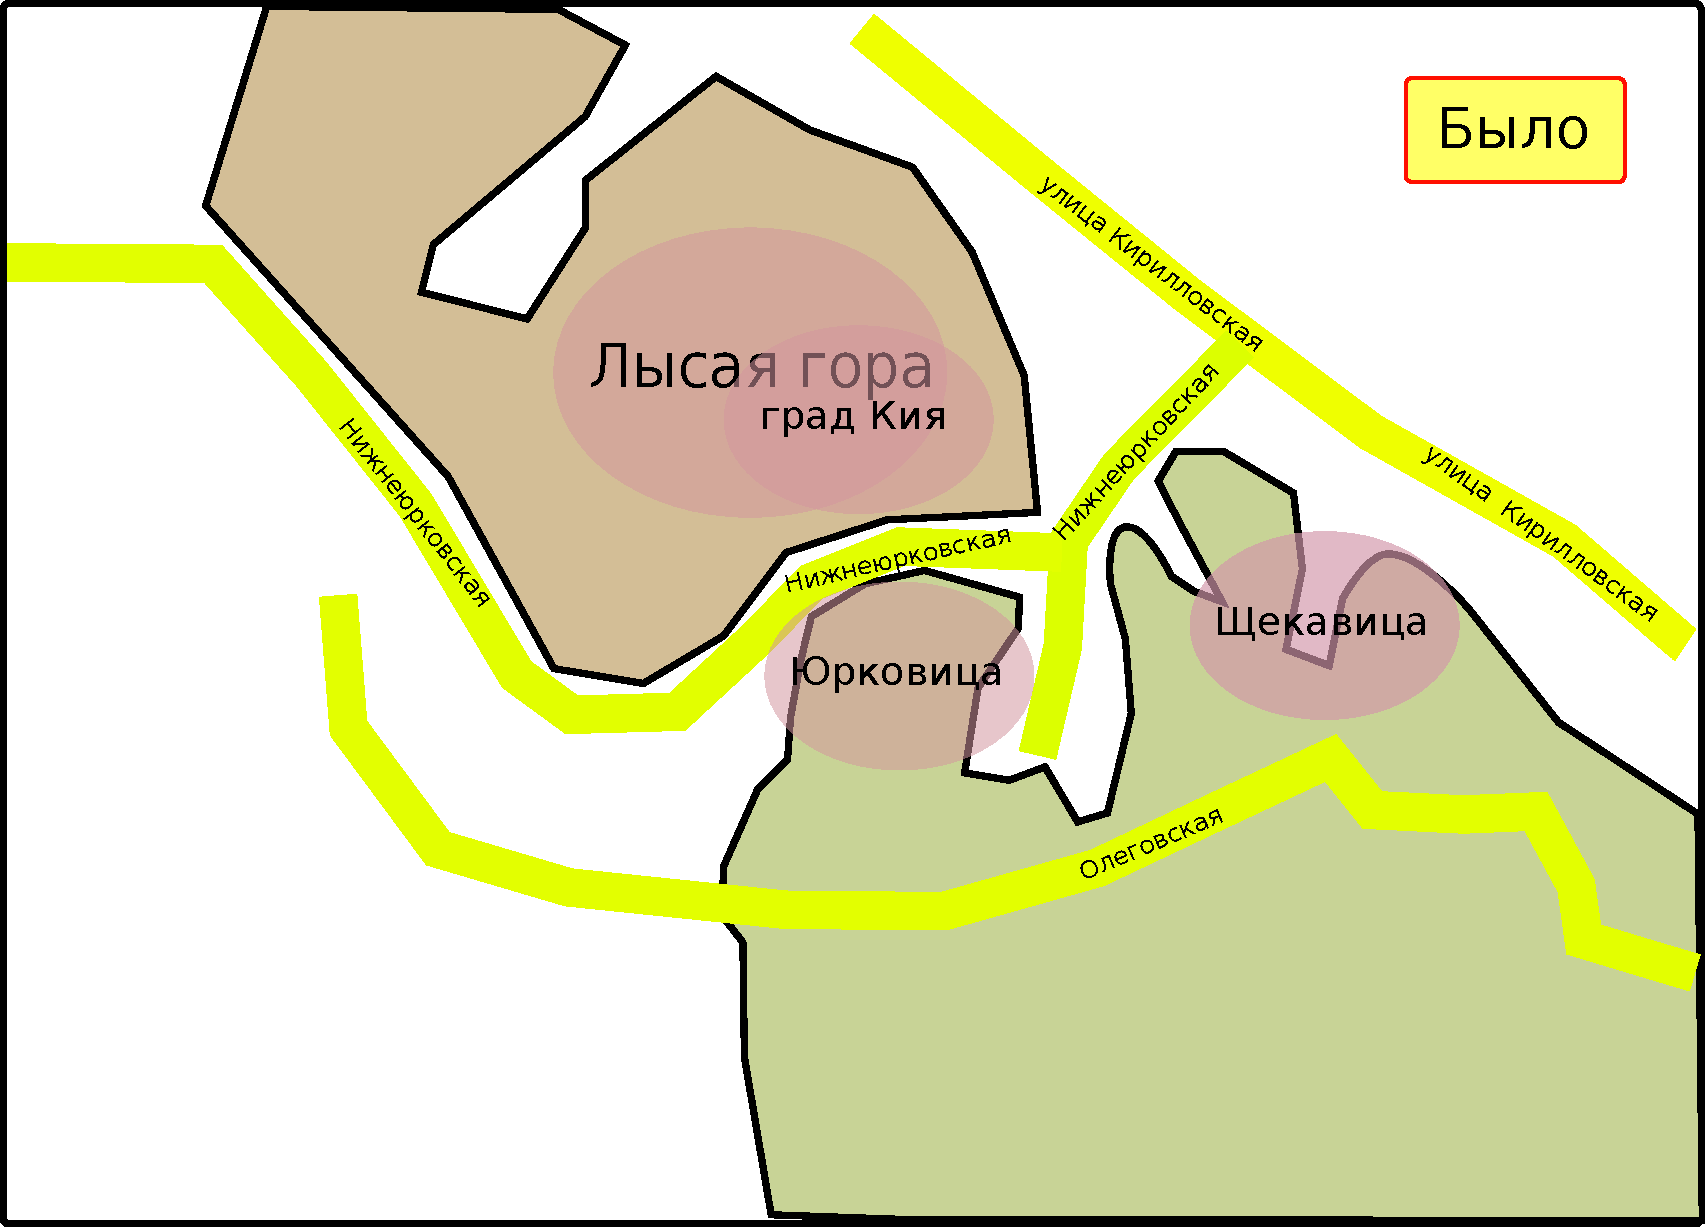
\includegraphics[width=0.90\linewidth]{chast-kirvys/poisk-yourk/yourk-bylo.pdf}
\end{center} 

\begin{center}
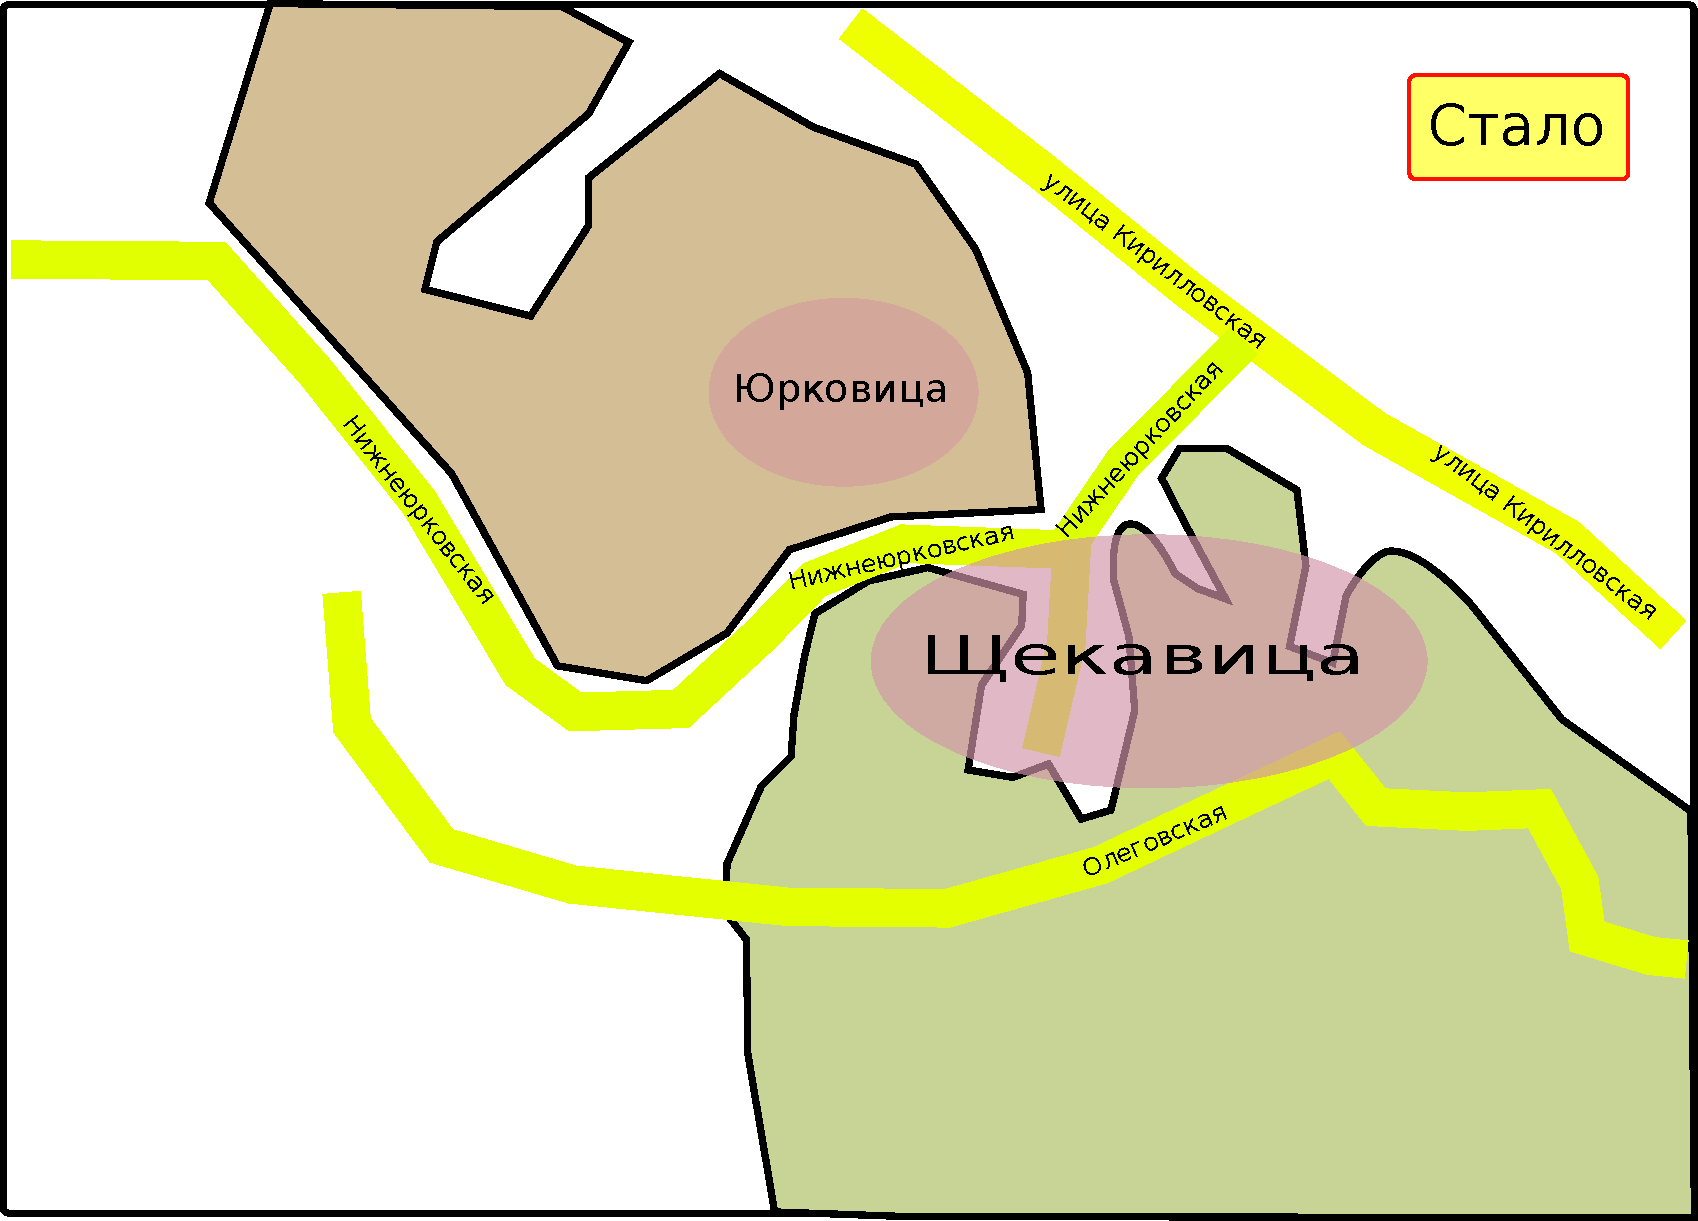
\includegraphics[width=0.90\linewidth]{chast-kirvys/poisk-yourk/yourk-stalo.pdf}
\end{center} 

Почему важно знать точно, какая гора является Юрковицей? Здесь несколько рассуждений, от истинности или ложности которых зависит всё. Первое – Юрковица это измененное название Хоревицы. Пока утверждаю голословно. Для удобства далее везде, где пишу Юрковица, подразумеваю и Хоревица. Коль Юрковицей считать Лысую гору, «град Киев» по картинке из Радзивилловской летописи смещается дальше на северо-запад от Лысой. А если полагать Юрковицей-Хоревицей гору, слывущую ныне отрогом Щекавицы, то град Кия приходится точно на бывшую Лысую гору («новую» Юрковицу), где найдены следы древнего городища.

Вспомним еще раз миниатюру из летописи.

\begin{center}
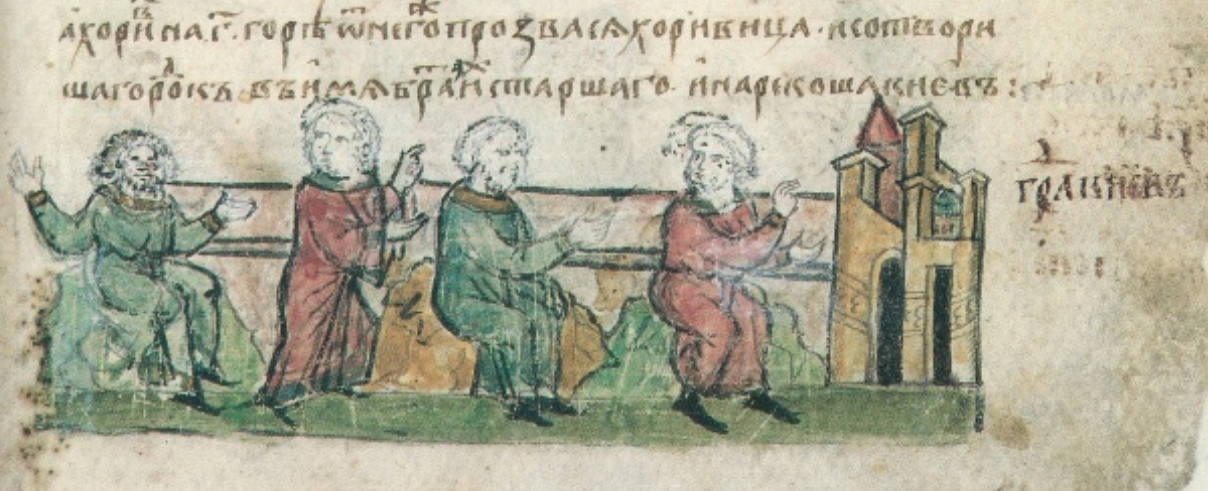
\includegraphics[width=\linewidth]{chast-kirvys/poisk-yourk/radz-tri-brata.jpg}
\end{center} 

Ежели смотреть на киевские холмы издалека с северо-востока, то третья по счету гора, Юрковица, на деле удалена от зрителя, в сравнении с Щекавицей и Лысой. Но художник развернул перспективу гор, поставив их на одной линии. Верно показано широкое удолье между Замковой (первая гора зеленого цвета) и Щекавицей (вторая гора, рыжая). 

Внимание! Не менее верно отражена и взаимосвязь Щекавицы с Юрковицей (третьей горой, зеленой), где обе являются частями одного холма. Если бы художник хотел нарисовать справа от Щекавицы Лысую гору, он бы сделал удолье между ними глубже и шире, разделив горы. Здесь же Щекавица и Хоревица изображены соединенными, эдакая гора о двух вершинах.

В том, что иллюстрация является картой, меня убеждает и, как я уже говорил, линия реки Лыбеди на заднем плане, и кое-что другое. Зеленая равнина под холмами – ведь это Подол и Плоская часть – Оболонь!

Слева на своем холме восседает старший брат Кий. Он не выглядывает из окошка расположенного справа «града Киева». Нет, он простодушно расставил руки – радуется! Сестра Лыбедь, да братья Щек и Хорив, все указывают руками на выстроенный в честь старшого град, отделенный от трех гор, справа от третьей, то бишь Хоревицы-Юрковицы.

Имя «Юрковица» переползло с одной горы на другую не только на картах. Из материалов дела Бейлиса, которое связано с Кирилловскими высотами, явствует, что Юрковицей уже в первом десятилетии 20 века называли местность по улице Верхне-Юрковской и примыкающей к ней части улиц Половецкой, Татарской. Кажется, имя Юрковицы распространялось вместе с названиями улиц – Большая Юрковская, Верхне-Юрковская, и так далее.

Как быть дальше? Как писать дальше книгу, если под Юрковицей с начала 20 века понимают бывшую Лысую гору, а Лысой горой считают Девич-гору за Теличкой?

Нельзя говорить – это название правильное, а это нет. Больше века Юрковицей считали другую гору. Название закрепилось за другой местностью в сознании не только краеведов, археологов, историков, но и местных жителей. А гора со старообрядческим кладбищем своё имя потеряла. Пустыри, заброшенные места лишаются имен, потому что людям нет смысла их вообще как-то называть.

Когда мы снимали серию «Киевской амплитуды» под названием «Возвращение в Логово змиево» и лезли на Лысую гору напротив исконной Юрковицы, то, обладая популярными знаниями, искренне считали, что поднимаемся на Юрковицу – Хоревицу. И бродя по древнему валу, предполагали, что тут обитал Хорив. Мы-то, думаю, верно сопоставили Юрковицу с Хоревицей, просто не подозревали, что давняя Юрковица – в другом месте!

Вот карта, согласно которой я буду излагать материал, относящийся к Юрковице и её окрестностям. Юрковица там, где старообрядческое кладбище. Щекавица там, где вышка, бывшая глушилка. То, что в народе слывет как «Юрковица», у меня – Лысая гора, иногда «новая Юрковица».

\begin{center}
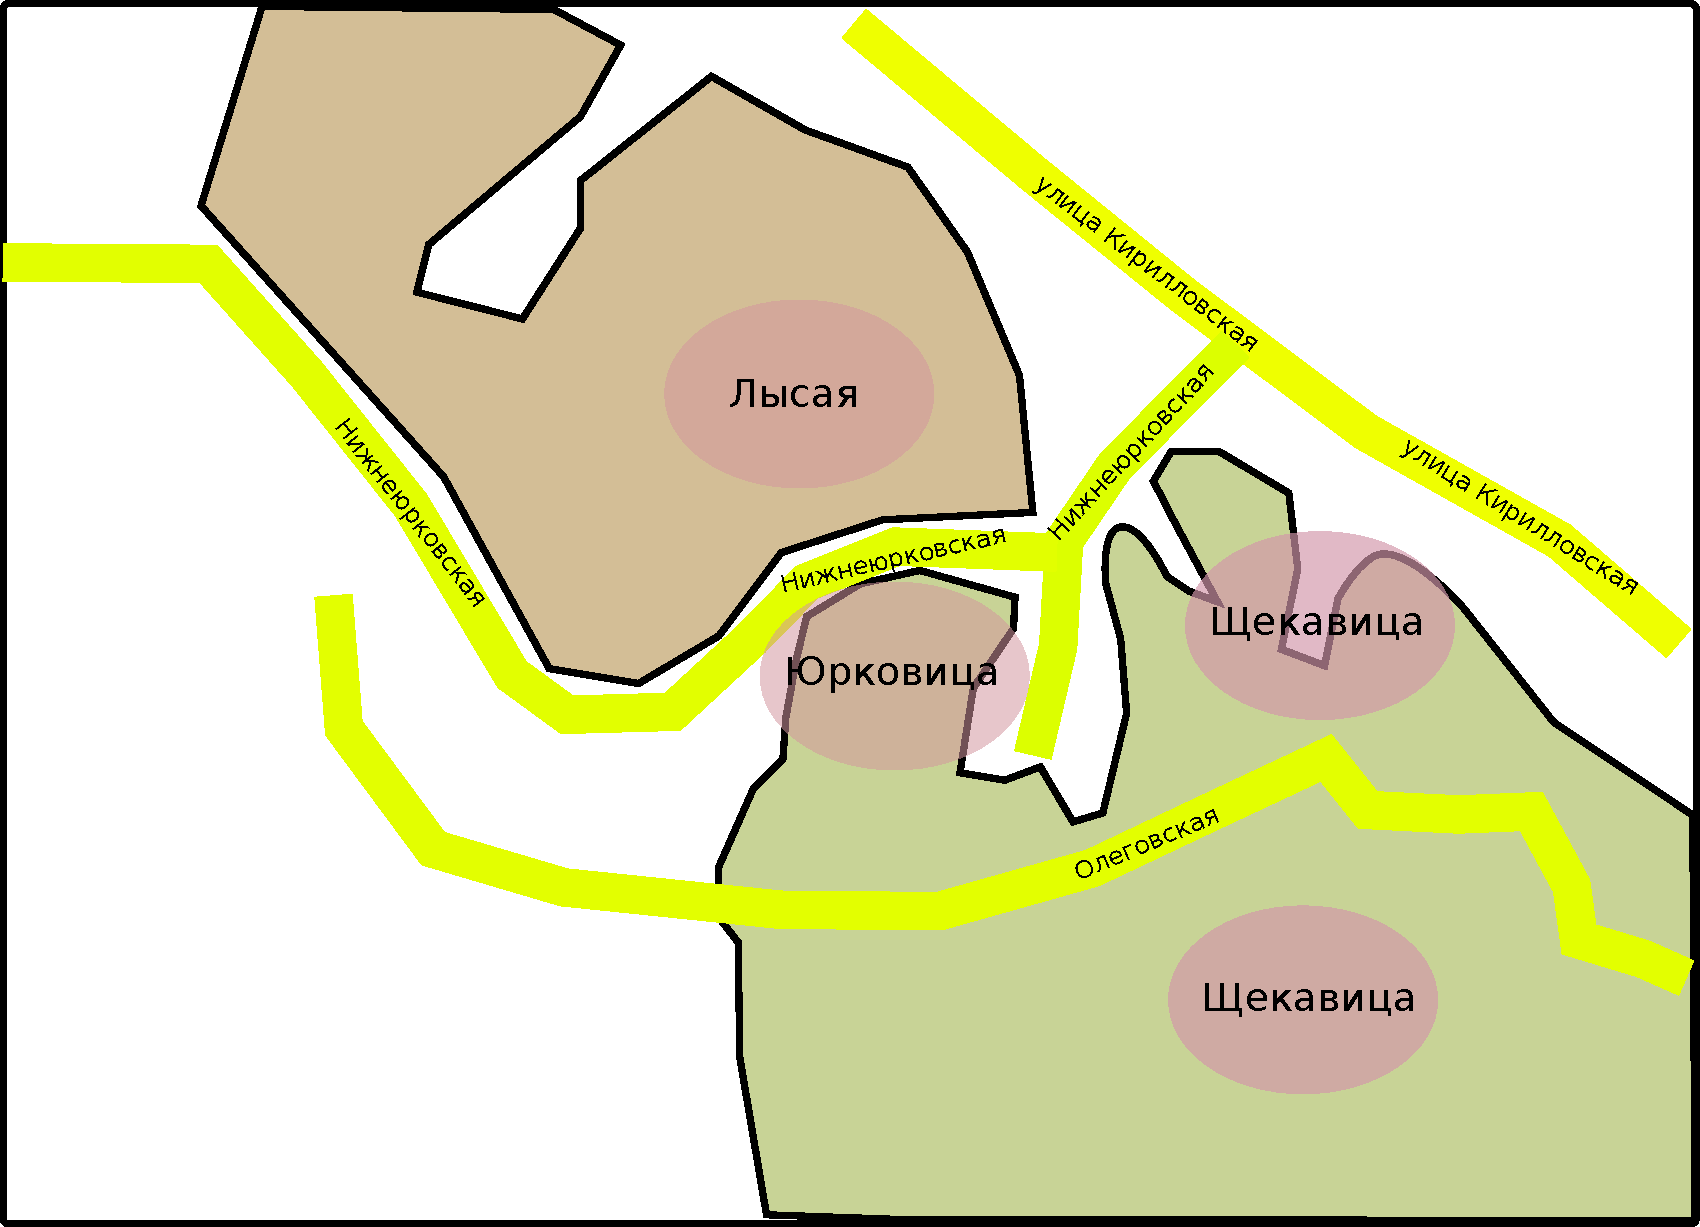
\includegraphics[width=\linewidth]{chast-kirvys/poisk-yourk/yourk-pravilno.pdf}
\end{center} 

В истинности обозначений на этой карте гор Лысой, Юрковицы и Щекавицы может убедиться каждый, кто посмотрит на старинные карты Киева и поднимет земельные акты. Лысой горы на старых картах впрочем нет, она так называлась во время, когда словесные описания заменяли подробные карты.

А как в других книгах и статьях про Киев? Как быть с различными краеведческими, археологическими трудами? Быть может, одни исследователи считали Юрковицей исконную Юрковицу, а другие – Лысую гору. И поди догадайся, в чем суть, если только не дана дополнительная привязка к местности, кроме «на Юрковице».

И без того хватает путаницы и неопределенности. Само слово «Юрковица» применительно к горе отсутствует в земельных актах 17-18 веков. В документах сначала возникает, в качестве земельной межи, Юрков ставок, а не «урочище Юрковица» или целая гора. Упоминается также, в середине 18 века, «поток Юрковиця». И потом мы видим уже гору Юрковицу на картах 19 века, но документы с таким названием за это время мне неизвестны.

Что за Юрко или Юрий такой был, с коим связан ставок, и отсылка ли это к Хориву, или, по другому списку летописи, Оуриву, вероятно «Юрию»? 

Хотя сомневаюсь, чтобы привязка ставка к личности сохранялась почти половину тысячелетия. С другой стороны, возможна обратная связь – от названия Хоревицы, которое с течением веков забылось, остался отголосок в имени ставка, а потом оно через ставок же возродилось, сначала как урочище, а потом распространилось на гору, уже как «Юрковица».

Подробности об Юрковом пруде читайте в главе «Юрков ставок», там же и рассуждения о первичности названия, способные немного поколебать задачу, которую я поставил себе в этих главах.

А задача такова – обосновать, почему на Лысой горе предполагаю место града Киева. Сама Юрковица играет тут роль ориентира, смежного с градом Киевом. Все интересные находки, по которым напрашивается вывод о древнем поселении, сделаны именно на Лысой. 

И несколько смущает соседство этой Лысой горы, понимаемой мною как «град Кия», с местностью «Лукьяновка», от названия которой довольно отбросить первые две буквы, и получится «Кияновка», если вместо «кья» произносить «кия».

Одну главу я отвожу описанию исконной Юрковицы. Затем мы отправимся по Лысой горе и улице Кирилловской, вдоль Кирилловских высот, с подробным разбором местности. Кирилловские высоты – уничтоженная сокровищница археологических памятников, каждый метр её уходит на тысячи лет в прошлое, а всякий замшелый кирпич или яма в земле тянет за собой переплетение историй, большей частью связанных с разрушением и смертью.

Здесь больше, чем где бы ни было в книге, я говорю о разных скелетах и костях, найденных археологами. И неожиданно поймал себя на мысли о странности в нашей системе ценностей и том, как принятое в обществе мнение об определенных вещах позволяет легко рассуждать о вещах тяжелых и обыденно воспринимать неприемлемое.

Если мы видим современную разоренную могилу, то возмущаемся вандализмом. А что раскапывают тысячи древних могил, принимается бездушно. Вроде не было таких живых людей, не носили они на шеях эти бусы, на пальцах кольца, и всё это добро их купно с останками извлекается из земли и нумеруется, заносится в каталоги, переносится в запасники различных музеев. Уважают покойников!

Завершая вводную главу про Юрковицу, не могу умолчать о неясном летописном предании. В Ипатьевском списке есть упоминание некой Серховицы, которую ученые нередко отождествляют с Юрковицей, не приводя к этому никаких оснований:

\begin{quotation}
6679. Сняшася братья\footnote{Союзники Андрея Боголюбского.} Вышегороде и, пришедше, сташа на Дорогожичи под святым Курилом Феодоровы недели, и второи недели оступиша весь град Киев. Мстиславу затворившюся в Киеве, бьяхуться из города, и бысть брань крепка отвсюду; Мстиславу изнемагающю в граде, Берендичи же и Торци льстяху под Мстиславом. 

И стояша 3 дни у города, и снидоша всих князий дружина Серховицею и ринушася к ним долов, у зад Мстиславу начаша стреляти. Мстиславу же начала дружина молвити: «что, княже, стоиши? поеди из города; нам их не перемочи». И поможе Бог Андреевичу Мстиславу с братьею, и взяша Киев.
\end{quotation}

Что сказано? Мстислав затворился в граде Киеве (это уже «традиционный» град Киев – Гора, там где София, Золотые ворота и так далее). И пока Мстислав сидит в городе, дружина всех князей спускается Серховицей и начинает стрелять «у зад Мстиславу».

Но ведь Мстислав – в городе, на Старокиевской горе! А где были князья до своего спуска Серховицей? На Дорогожичах под Кирилловским монастырем, а затем окружили весь Киев. И где-то в пределах окружения, сойдя Серховицей, зашли Мстиславу, который в городе, в тыл. Что же считать тылом? Тогда можно будет догадаться, что подразумевал летописец под Серховицей.

Однако надо же понимать, что спустившись по Нижнеюрковской, как думают ученые, уравнивая Серховицу и современную Юрковицу (точнее, овраг по Нижнеюрковской улице), князья никак не могли стрелять «у зад Мстиславу». Но ученые не представляют себе местности или не хотят этого делать, и говорят – Серховица это Юрковица. Одни из Серховицы выкидывают буквы, другие добавляют, придумывают некое «древнерусское слово» – обычное жонглирование. 

Как по мне, что «Серховица» больше всего похоже на искаженное «Церковица». Так хотя бы осмысленно. А где она была, не знаю.
